\question \textbf{Bitvector compression}

\begin{parts}
\part Given the following Bitvector
\begin{align*}
    B = \left[11010010\,11010001\,01011111\,01110001\,10101000\,00101100\right]
\end{align*}
compute the compressed representation of $B$ with block length $b = 4$, as an array $C[1, ⌈n/b⌉]$, where $C[i] = c_i$ is the class that describes a block with i number of 1s, and an array $O[1, \lceil n/b\rceil]$, where $O[i] = o_i$ is the offset that identifies which element $i$ is among those of its class $c_i$.
When encoding the offsets, follow the technique presented in the lecture on slide 2055.

\begin{solution}

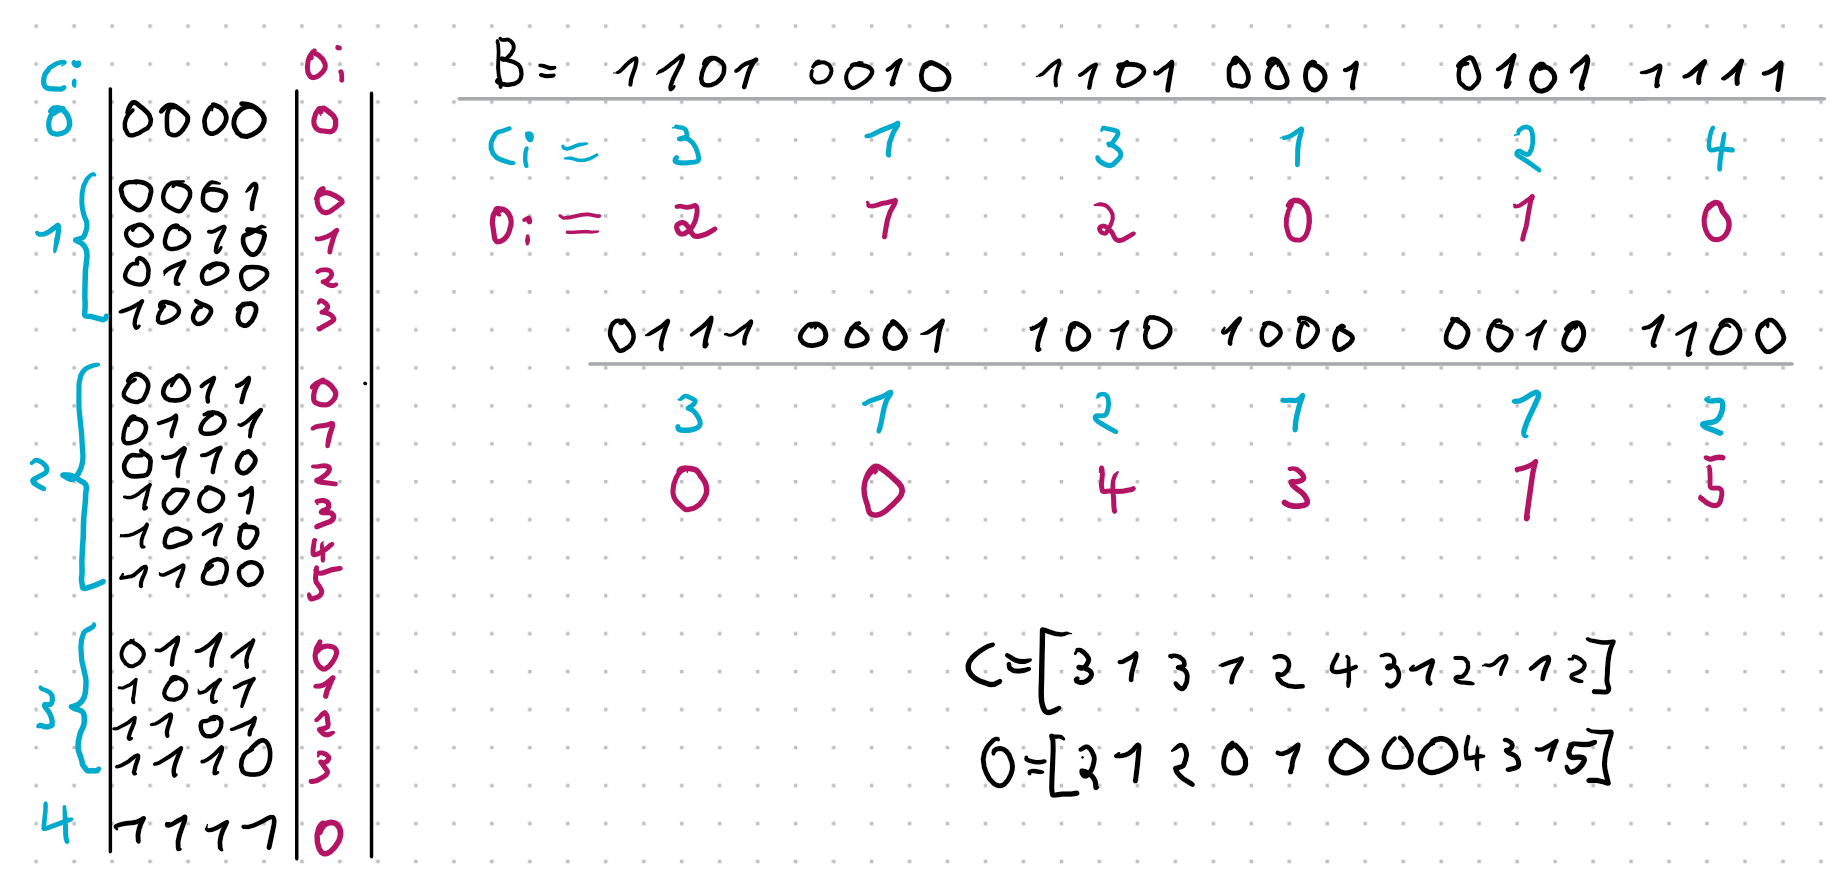
\includegraphics[width=\linewidth]{task_2/a2_a.png}
\end{solution}


\part Decompress the following code into a Bitvector:
\begin{align*}
    b =4,\,C=[1,3,2,1],\,O=[0,3,2,2]
\end{align*}


\begin{solution}

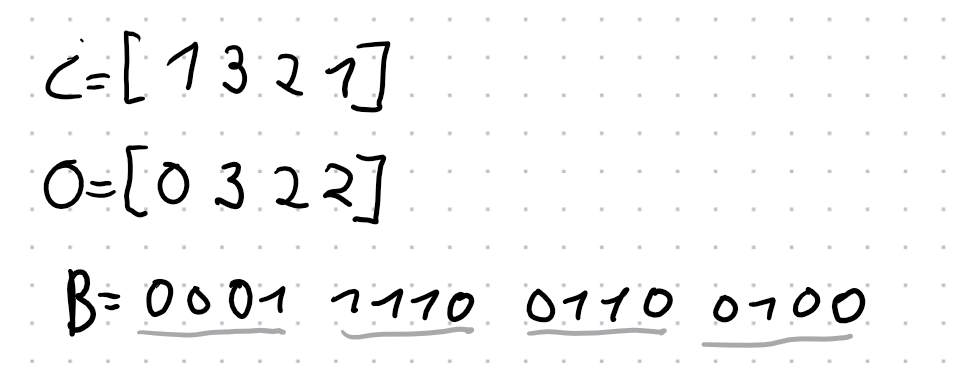
\includegraphics[width=0.4\linewidth]{task_2/a2_b.png}
\end{solution}

\end{parts}


% For tasks without simply remove the \begin{parts}...\part...\end{parts} commands